\documentclass[../Article_Model_Parameters.tex]{subfiles}
\graphicspath{{\subfix{../Figures/}}}
\begin{document}
	
	This study investigates the extraction of essential oil from chamomile flowers (Matricaria chamomilla L.) via supercritical fluid extraction techniques and modelling of this process. Chamomile is a medicinal herb widely cultivated in southern and eastern Europe—such as Germany, Hungary, France, and Russia. It can be found outside of Europe in Brazil as discussed by \citet{Singh2011}. This plant is distinguished by its hollow, bright gold cones, housing disc or tubular florets and surrounded by about fifteen white ray or ligulate florets. Chamomile has been used for its medicinal benefits, serving as an anti-inflammatory, antioxidant, mild astringent, and healing remedy. Chamomile's aqueous extract is widely used as a gentle sedative to calm nerves and mitigate anxiety, hysteria, nightmares, insomnia, and other sleep-related conditions, according to \citet{Srivastava2009}. \citet{Orav2010} reported that oil yields from dried chamomile samples ranged from 0.7 to 6.7 mL/kg. Notably, the highest yields of essential oil, between 6.1 and 6.7 mL/kg, were derived from chamomile sourced from Latvia and Ukraine, while chamomile from Armenia exhibited a lower oil content of 0.7 mL/kg.
	
	%The present study focuses on extracting essential oil from the chamomile flowers with supercritical fluid extraction and modelling that process. Caraway is a biennial plant belonging to the Apiaceae family. It is widespread in Asia, Europe, and North Afri``ca. The essential oil obtained from caraway finds its potential application as a fragrance ingredient in perfumes, liquors, and toothpaste. As presented by \citet{Hromis2015}, the dried caraway contains nearly~2.8–5\% essential oil, from which the main compounds are carvone, pinene, camphene, limonene, and carveol. 
	
	%The economic feasibility of the process is crucial when selecting the appropriate technology. Conventional processes, such as distillation and organic solvent extraction, are frequently used for essential oil extraction. The distillation process is carried out at a high temperature, which causes thermal degradation of thermolabile compounds—considering that alternative techniques like supercritical fluid extraction gained popularity for extraction. Supercritical carbon dioxide, in particular, is attractive due to its unique properties such as being inflammable, non-toxic, low critical temperature, and non-corrosive. Furthermore, its critical point is relatively low compared to other fluids, making it a suitable alternative to traditional extraction techniques. The supercritical fluids exhibit both gas- and liquid-like properties so that operating conditions can adjust the dissolving power.
	
	%Various mathematical models have been proposed to describe the extraction of valuable compounds from a fixed biomass bed. However, selecting an appropriate extraction model requires understanding the physical phenomena occurring in the operational unit. Each model has its own set of assumptions and describes different mass transfer mechanisms and equilibrium relationships.
	
	%One model proposed by \citet{Reverchon1993} is the hot ball model, which is based on an analogy to heat transfer and describes an extraction process from solid particles containing small quantities of solute where solubility is not a limiting factor. 
	
	%Another model, the Broken-and-Intact Cell model, was presented by \citet{Sovova1994}. This model describes a system where the outer surfaces of particles have been mechanically interrupted, allowing easy access of solvent to the solute from the broken cells. In contrast, the solute from the intact cells is less accessible due to high mass transfer resistance.
	
	%\citet{Reverchon1996} developed a model for fluid-solid extraction, where the oil is treated as a single component, and the extraction process is controlled by internal mass transfer resistance, neglecting external mass transfer. However, this model does not consider the influence of axial dispersion or changes in fluid density and flow rate along the bed.
	
	%In this work, the fundamental governing equations are derived and combined with the kinetic model suggested by \citet{Reverchon1996} to obtain a general model for the oil extraction process from the chamomile flower. This model simplifies some of the physical behaviour to obtain a control-oriented model. It is assumed that the extraction process operates semi-continuously in a cylindrical vessel. The solvent is first brought to supercritical conditions, pumped through a fixed bed of finely chopped biomass, and the solute is extracted from the biomass. The solvent and solute are then separated in a flush drum, and the extract is collected. The feed flow rate ($F_{in}$) and inlet temperature ($T_{in}$) of the extractor can be measured and manipulated, while the vessel pressure ($P$) can also be measured and manipulated. However, the outlet temperature ($T_{out}$) can only be measured. Figure \ref{fig: SFE_drawing} shows a simplified flow diagram.
	
	Evaluating the economic viability of the process is essential when choosing the suitable technology for essential oil extraction. Traditional methods, such as distillation and organic solvent extraction, are commonly employed but come with drawbacks. Distillation, for example, involves high temperatures that can lead to the thermal degradation of heat-sensitive compounds. This limitation has led to the increased popularity of alternative techniques like supercritical fluid extraction. Supercritical carbon dioxide is particularly appealing due to its distinctive properties: it's inflammable, non-toxic, has a low critical temperature, and is non-corrosive. Moreover, its relatively low critical point, compared to other fluids, positions it as an advantageous alternative to conventional extraction methods. Supercritical fluids are capable of exhibiting both gas- and liquid-like properties, allowing for adjustable dissolving power through changes in operating conditions.
	
	The literature offers a variety of mathematical models aimed at detailing the extraction of valuable compounds from a fixed biomass bed. Selecting a fitting model necessitates a deep understanding of the physical processes at play within the operational unit, as each model is built on specific assumptions and outlines distinct mass transfer mechanisms and equilibrium dynamics.
	
	One model proposed by \citet{Reverchon1993} is the hot ball model, which is based on an analogy to heat transfer and describes an extraction process from solid particles containing small quantities of solute where solubility is not a limiting factor.
	
	The Broken-and-Intact Cell model, proposed by \citet{Sovova1994}, assumes that external surfaces of particles are mechanically disrupted, allowing the solvent's access to the solute in broken cells, while the solute in intact cells remains less accessible due to higher mass transfer resistance.
	
	\citet{Reverchon1996} formulated a fluid-solid extraction model where the solute is treated as a single component, governed by internal mass transfer resistance and omitting the effects of external mass transfer, axial dispersion, and variations in fluid density and flow rate throughout the bed.
	
	This work builds upon the linear kinetic model suggested by \citet{Reverchon1996}, deriving fundamental governing equations to develop a comprehensive model for the chamomile oil extraction process. This model aims for control-oriented simplicity, assuming a semi-continuous operation within a cylindrical vessel. The process involves supercritical solvent being pumped through a fixed bed of finely chopped biomass to extract the solute, followed by separation of the solvent and solute in a flush drum to collect the extract. Parameters such as the feed flow rate ($F_{in}$) and inlet temperature ($T_{in}$) are adjustable and measurable, as is the vessel pressure ($P$), whereas the outlet temperature ($T_{out}$) can only be monitored. A simplified flow diagram is presented in Figure \ref{fig: SFE_drawing}, illustrating the process setup.
	
	\begin{figure}[h!]
		\centering
		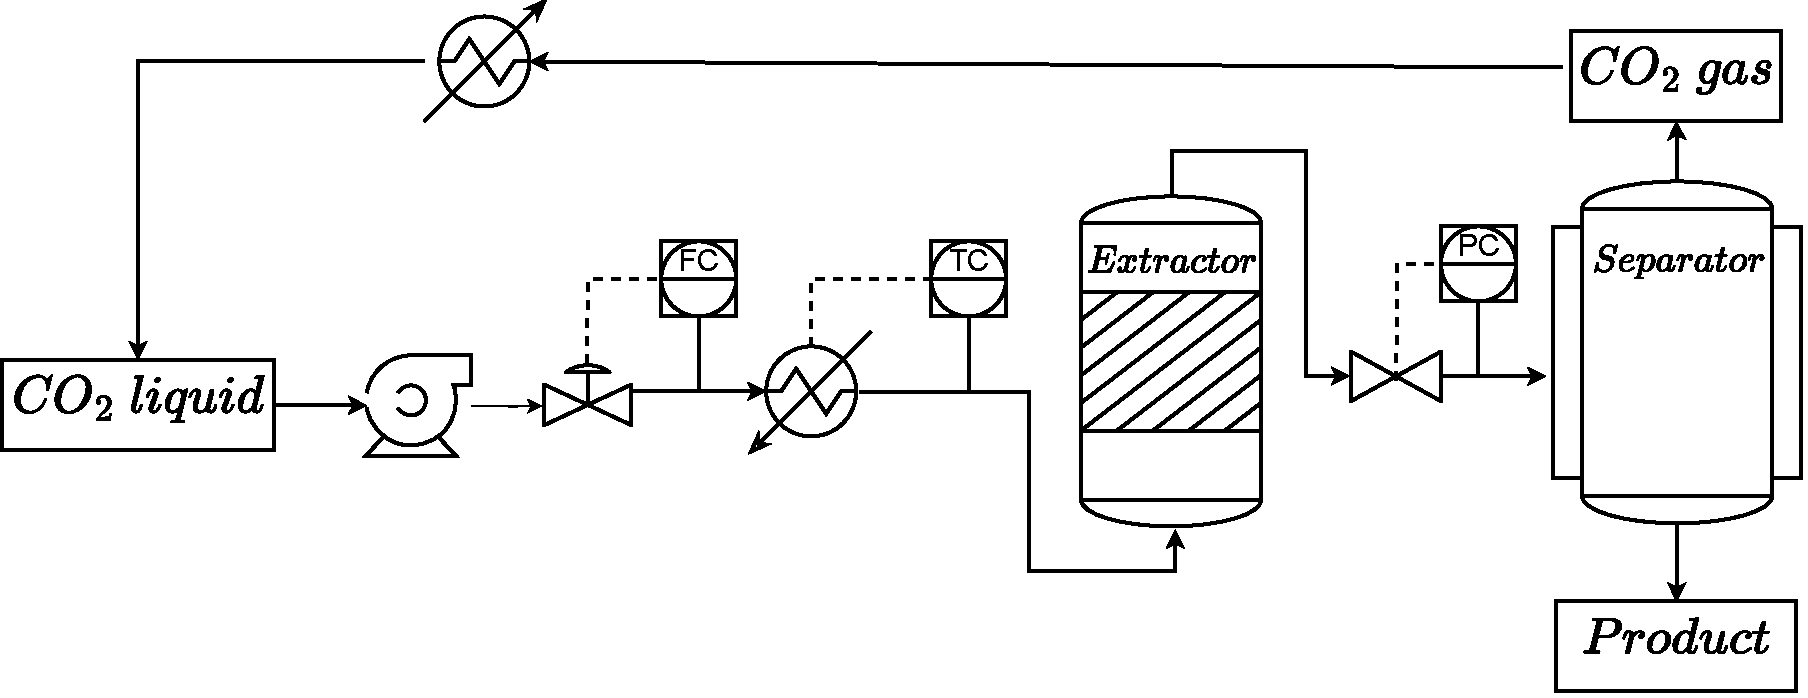
\includegraphics[width=\columnwidth]{Figures/PFD.drawio.pdf}
		\caption{Process flow diagram}
		\label{fig: SFE_drawing}
	\end{figure}

	%This study aims to develop a process model for extracting natural substances from solid materials and liquids using supercritical fluids, specifically supercritical $CO_2$. To achieve this, the solvent properties are estimated based on thermodynamic relations, and the extraction kinetic parameters are estimated based on a set of experiments conducted under various conditions. The maximum likelihood estimator is used to solve the parameter estimation problem, and the obtained parameters are subjected to regression to derive correlations. These correlations enable the process model to be generalized across a range of temperatures (40 to $50~^\circ C$) and pressures (200 to 300 bar).
	
	%The study is structured as follows: Chapter \ref{CH: Thermodynamic} provides a general discussion on supercritical fluids to familiarize the reader with their properties. Chapter \ref{CH:Governing_equations_chapter} introduces the general balance equations. The balance equations are combined with the extraction kinetic equation to develop the process model in Chapter \ref{CH: Extraction_model}. The maximum likelihood technique is presented in Chapter \ref{CH: Parameter_estimation} and is then combined with the process model. Chapter \ref{CH: Experiments} describes the experimental work and the data collected from experiments, which are used to estimate missing parameters related to the extraction kinetics. Finally, the parameter estimations and simulation results are discussed in Chapters \ref{CH: Results} and \ref{CH: Conclusion}.
		
	This study focuses on creating a process model for the extraction of natural substances from solid materials using supercritical fluids, with a particular emphasis on supercritical $CO_2$. The approach involves estimating the solvent properties through thermodynamic relationships and determining the extraction kinetic parameters via a series of experiments conducted under a variety of conditions. The maximum likelihood estimator method is employed to address the parameter estimation challenge, with the derived parameters subsequently used to establish correlations. These correlations are instrumental in extending the applicability of the process model across different temperatures (30 to 40$^\circ C$) and pressures (100 to 200 bar).
	
	%The organization of the study is as follows: Chapter \ref{CH: Thermodynamic} offers an overview of supercritical fluids, aiming to acquaint the reader with their unique properties. 
	Chapter \ref{CH:Governing_equations_chapter} outlines the fundamental balance equations. These equations are then integrated with the extraction kinetic equation in Chapter \ref{CH: Extraction_model} to formulate the process model. Chapter \ref{CH: Parameter_estimation} introduces the maximum likelihood estimation technique, which is subsequently applied within the context of the process model. Chapter \ref{CH: Experiments} details the experimental procedures and the data acquisition necessary for estimating the kinetic parameters related to the extraction process. The study culminates in Chapters \ref{CH: Results} and \ref{CH: Conclusion}, where the parameter estimations and simulation outcomes are thoroughly analysed and discussed.
		
\end{document}